%!TEX root = Thesis.tex
\chapter{State of the Art}
The following chapter covers an overview and analysis of the existent solutions in
the related research areas of web-based third-party applications, which were designed specially for retrieving differet type of sensed data to the user application. At the beginning the prominent examples of dashboards platforms are studied and evaluated against the requirements described in the previous chapter with a purpose to clarify their personalized capabilities.
 Since the thesis is targeted at the creation of generic frontend, 

\section{Mashups Development Platforms}
A growing popularity of mashup\footnote{\url{http://www.programmableweb.com/ applications}} applications, that is evidenced by a large amountof currently existent mashups, is accompanied by the rapidly increasing number of
mashups development tools and platforms \cite{taivalsaari2009mashware, koschmider2009elucidating, daniel2010toward, aghaee2012reusable}. Both commercial products and research prototypes have a broad range of features that
simplify a mashups design process, and provide mashups storage and publication.
One of the prominent consumer mashup tool is Yahoo Pipes\footnote{\url{http://pipes.yahoo.com/pipes/}}, which allows to create new data mashups via a visual editor by mixing different feed types. Another example is DERI Pipes\footnote{\url{http://pipes.deri.org/}} tool, which is similar to Yahoo Pipes, but enhanced with the possibility to handle the Resource Description
Framework (RDF) format. Different from the data pipes Intel Mash Maker\footnote{\url{http://software.intel.com/en-us/articles/intel-mash-maker-mashups-for-the-masses}} is implemented as a web browser’s extension. While browsing a web page, the Mash
Maker toolbar suggests possible additions, e. g. widgets, to the current page, which
extend its capabilities and provide addition information from the other web sites.

\section{Portal Development Platforms}
Many of the Web applications seen today incorporate different patterns to merge
functionality directed toward the end user. Many of them started out not being
portals, but evolved into portals as functionality was added.
This section focuses on the design approaches for portal solutions. 
It addresses the design stage of the solution development process, highlighting the key issues that are specific to portal and
application designs\cite{pautasso2008restful,seong2006usability}.

\begin{enumerate}
\item Object-Oriented design patterns, including Model-View-Control design
\item Portlet framework design
\end{enumerate}
\subsection{Model-View-Control Pattern}
In the design shown in Figure 1 on page 8, Model represents the application
object that implements the application data and business logic. The View is
responsible for formatting the application results and dynamic page construction.
The Controller is responsible for receiving the client request, invoking the
appropriate business logic, and based on the results, selecting the appropriate
view to be presented to the user.
The Model represents enterprise data and the business rules that govern
access to and updates to this data. Often the Model serves as a software
approximation to a real-world process, so simple real-world modeling
techniques apply when defining the Model.
A View renders the contents of a Model. It accesses enterprise data through
the Model and specifies how that data should be presented.
It is the View's responsibility to maintain consistency in its presentation when
the Model changes. This can be achieved by using a push Model, where the
View registers itself with the Model for change notifications, or a pull Model,
where the View is responsible for calling the Model when it needs to retrieve
the most current data.
A Controller translates interactions with the View into actions to be performed
by the Model. In a stand-alone GUI client, user interactions could be button
clicks or menu selections, whereas in a Web application, they appear as GET
and POST HTTP requests. The actions performed by the Model include
activating business processes or changing the state of the Model. Based on
the user interactions and the outcome of the Model actions, the Controller
responds by selecting an appropriate View.
\begin{figure}[!ht]
\centering
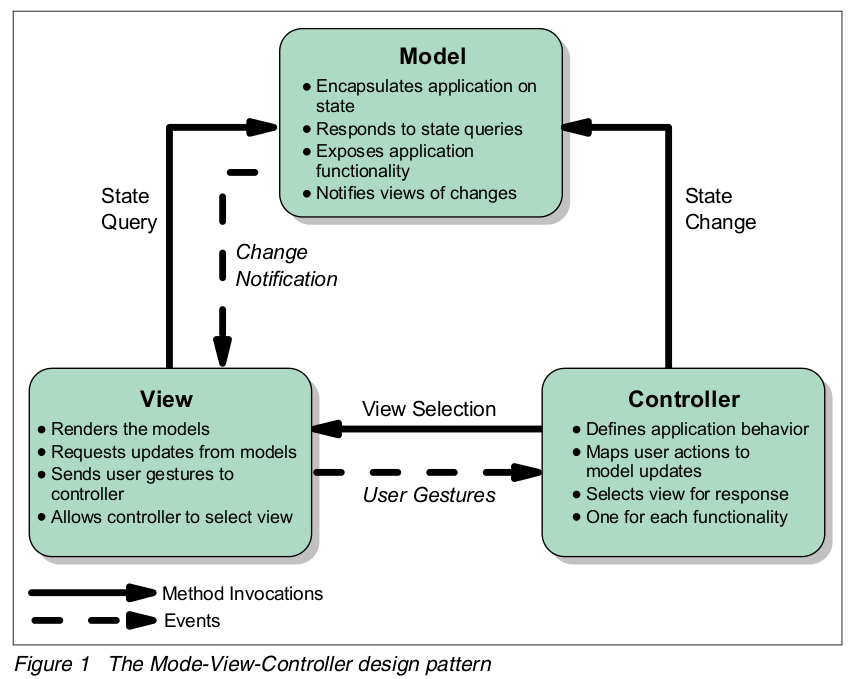
\includegraphics[scale=0.7]{images/MVCPattern.png}   
\caption[MVC Pattern]{MVC Pattern}
\label{img:MVCPattern}                           
\end{figure}
%\footnotetext{Image taken from \url{blog.csdn.net/cain/article/details/6617173}}
\subsection{Portlet Framework Design}

\section{Browser Based Collaborative Systems}

\section{Non-Browser Based Collaborative Systems}

\section{Summary}
This chapter briefly introduced main approaches for building web-based dashboards by retriving sensed data. Main focus was given to its multy-user usability, adaptive UI design, dynamic content composition.
